\documentclass[12pt,letterpaper]{article}
% the package for network diagram
\usepackage{tikz-network}
% the package for the Axis plot
\usetikzlibrary{shapes}
\usepackage{pgfplots}
% the package for fill color in Axis Plot
\usepgfplotslibrary{fillbetween}
% Matlab code package
\usepackage[framed,numbered,autolinebreaks,useliterate]{mcode}

\usepackage[english]{babel} 
\usepackage[utf8]{inputenc}	
\spanishdecimal{.}
% \usepackage{amsmath,amsthm,amsfonts,amssymb,amscd}
\usepackage{amsmath,amsfonts,amssymb,amscd,amsthm}

%Theorem Package
\newtheorem{theorem}{Theorem}
\usepackage{multirow,booktabs}
\usepackage[table]{xcolor}
\usepackage{fullpage}
\usepackage{lastpage}
\usepackage{enumitem}
\usepackage{fancyhdr}
\usepackage{mathrsfs}
\usepackage{wrapfig}
\usepackage{setspace}
\usepackage{calc}
\usepackage{multicol}
\usepackage{cancel}
\usepackage[retainorgcmds]{IEEEtrantools}
\usepackage[margin=2.5cm]{geometry}
\usepackage{floatrow}
\newlength{\tabcont}
\setlength{\parindent}{0.0in}
\setlength{\parskip}{0.05in}
\title{TALLER ALGEBRA LINEAL ISAAC RODRIGUEZ}
\newcommand\course{Soft Computing ENGG6570}	
\newcommand\semester{2021} 
\newcommand\yourname{Yaowen Mei}  
\theoremstyle{definition}
\newtheorem{defn}{Definición}
\newtheorem{reg}{Regla}
\newtheorem{ejer}{EJERCICIO}
\pagestyle{fancyplain}
\headheight 32pt
\lhead{\yourname\ \vspace{0.05cm} \\ \course}
\chead{\textbf{\Large Homework-1}}
\rhead{2021/05/28}

%% QED in black square
\renewcommand{\qedsymbol}{\hfill\blacksquare}
\newcommand{\qedwhite}{\hfill \ensuremath{\Box}}
%% Proof and Lamma
\newtheorem{lemma}[theorem]{Lemma}

\begin{document}
\textbf{Question 1-1}.\textbf{Write the feedforward equations of h1, h2, h3 and y, as a function of the input
variables x1, x2 and x3. Note that the thresholds must be included:}
\begin{center}
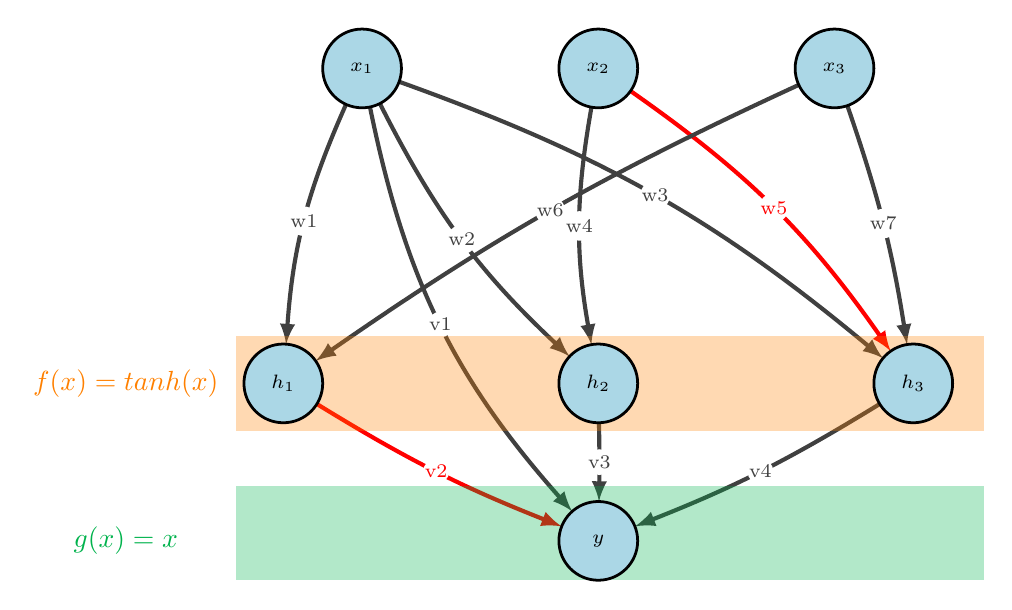
\begin{tikzpicture}
% \Vertex[x=0,size=1,RGB,color={190,174,212},label=$x_0\equiv1$]{TI} 
\Vertex[x=3,size=1,label=$x_1$]{A} 
\Vertex[x=6,size=1,label=$x_2$]{B} 
\Vertex[x=9,size=1,label=$x_3$]{C}
% The orange Box
\Plane[x=-4.6,y=1.4,width=1.2,height=9.5,color=orange, NoBorder]
\Text[x=0,y=-4.0,fontsize=\SMALL,color=orange]{$f(x)=tanh(x)$}
% \Vertex[x=0,y=-4,size=1,RGB,color={190,174,212},label=$h_0\equiv1$]{TH}
\Vertex[x=2,y=-4,size=1,label=$h_1$]{D} 
\Vertex[x=6,y=-4,size=1,label=$h_2$]{E}
\Vertex[x=10,y=-4,size=1,label=$h_3$]{F}
% The Green Box
\Plane[x=-6.5,y=1.4,width=1.2,height=9.5,color=green!70!blue, NoBorder]
\Text[x=0,y=-6,fontsize=\SMALL,color=green!70!blue]{$g(x)=x$}
\Vertex[x=6,y=-6,size = 1,label=$y$]{Z}

\Edge[bend=-10,Direct=true,label=w1](A)(D)
\Edge[bend=-10,Direct=true,label=w2](A)(E)
\Edge[bend=10,Direct=true,label=w3](A)(F)

\Edge[bend=-10,Direct=true,label=w4](B)(E)
\Edge[bend=10,Direct=true,color=red,label=w5](B)(F)
\Edge[bend=-5,Direct=true,label=w6](C)(D)
\Edge[bend=5,Direct=true,label=w7](C)(F)

\Edge[bend=-5,Direct=true,color=red,label=v2](D)(Z)
\Edge[bend=1,Direct=true,label=v3](E)(Z)
\Edge[bend=5,Direct=true,label=v4](F)(Z)
\Edge[bend=-15,Direct=true,label=v1](A)(Z)
\end{tikzpicture}
\end{center}
\\
\textbf{Solution 1-1:} 
\\
Directly read from the diagram above, for hidden layer, we can write:
\begin{equation}
    \boxed{{h_{ & 1}} = f\left( {{w_1}{x_1} + {w_6}{x_3} + \theta_{h1} } \right)}
\end{equation}
    
\begin{equation}
    \boxed{{h_{ & 2}} = f\left( {{w_2}{x_1} + {w_4}{x_2} + \theta_{h2} } \right)}
\end{equation}

\begin{equation}
    \boxed{{h_{ & 3}} = f\left( {{w_3}{x_1} + {w_5}{x_2} + {w_7}{x_3} + \theta_{h3} } \right)}
\end{equation}

For the output layer, we can write:
\begin{equation}
  y = g\left( {{v_1}x{ & _1} + {v_2}{h_1} + {v_3}{h_2} + {v_4}{h_3}} \right)\label{eq-1-1-4}  
\end{equation}

\textbf{Question 1-2}. \textbf{Derive a learning algorithm for v2, w5, using LMS (Least Mean Square)
method, i.e., by minimizing the output error e = t - y, where t is the target output.}
\\

\\
\textbf{Solution 1-2:}
\\
Given that $f(x)=tanh(x)$ and $g(x)=x$, we have $f'$ and $g'$:
\[f' = 1 - {f^2}\]
\[g' = 1\]

By observation from the diagram, $v_2$ is a directed Edge from Vertex $h_1$ to Vertex $y$; while, $w_5$ is a directed Edge from Vertex $x_2$ to $h_3$.

From the lecture, we can proofed that the LMS Error strategy leads to a uniform learning equation for both the hidden layer and the output layer:
\clearpage

\[\Delta Edge = \eta  \times \underbrace {{{\left( {Activation Function} \right)}^\prime }}_{{\rm{Activation function @ Dist}}} \times \underbrace {\left( {error} \right)}_{{\rm{error @ Dist}}} \times \underbrace {\left( {input} \right)}_{{\rm{value @ Source}}}\]


\begin{equation}
     \boxed{\Delta {v_2} = \eta g'{e_y}{h_1}  = \eta \left( {t - y} \right){h_1}}\label{eq1-2-1}
\end{equation}


\begin{equation}
    \boxed{\Delta {w_5} = \eta f'{e_{h3}}{x_2} = \eta \left( {1 - {f^2}} \right){e_{h3}}{x_2}}\label{eq1-2-2}
\end{equation}


Where:
\[{e_{h3}} = g' \times e \times {v_4} = g'\left( {t - y} \right){v_4} = \left( {t - y} \right){v_4}\]
\noindent{\color{red} \rule{\linewidth}{0.25mm}}
% ==========================================================================================
The following details are given if one is interested in seeing the mathematical details for getting equation \eqref{eq1-2-1}, and equation \eqref{eq1-2-2} directly from the defination of $E$:

The LMS Error $E$ is defined as:
\[E = \frac{1}{2}{\left( {t - y} \right)^2}\]

It is trivial to proof equation \eqref{eq1-2-1}, $\Delta{v_2}= \eta \left( {t - y} \right){h_1}$, from the definition of $E$:
\[\Delta {v_2} =  - \eta \frac{{\partial E}}{{\partial {v_2}}} =  - \eta \left( {t - y} \right)\left( {\frac{{\partial \left( {t - y} \right)}}{{\partial {v_2}}}} \right) = \eta \left( {t - y} \right)\left( {\frac{{\partial y}}{{\partial {v_2}}}} \right) = \eta \left( {t - y} \right)\left( {{h_1}g'} \right) = \eta \left( {t - y} \right){h_1} \qed\]
It is tricky to proof equation \eqref{eq1-2-2} from the definition of $E$.
\\
One can write:
\begin{equation}
  \Delta {w_5} =  - \eta \frac{{\partial E}}{{\partial {w_5}}} =  - \eta \left( {t - y} \right)\left( {\frac{{\partial \left( {t - y} \right)}}{{\partial {w_5}}}} \right) = \eta \left( {t - y} \right)\left( {\frac{{\partial y}}{{\partial {w_5}}}} \right)  \label{eq1-2-3}
\end{equation}
Using equation \eqref{eq-1-1-4} to re-write $y$ in equation \eqref{eq1-2-3} so that $y$ explicitly contains $w_5$:
\[y = g\left( {{v_1}x{ & _1} + {v_2}{h_1} + {v_3}{h_2} + {v_4}{h_3}} \right) = g\left[ {\left( {{v_1}x{ & _1} + {v_2}{h_1} + {v_3}{h_2}} \right) + {v_4}f\left( {{w_3}{x_1} + {w_5}{x_2} + {w_7}{x_3} + {\theta _{h3}}} \right)} \right]\]

\begin{equation}
   \frac{{\partial y}}{{\partial {w_5}}} = g'\frac{    {\partial \left[ { \left( {{v_1}x{ & _1} + {v_2}{h_1} + {v_3}{h_2}} \right) + {v_4}f\left( {{w_3}{x_1} + {w_5}{x_2} + {w_7}{x_3} + {\theta _{h3}}} \right)} \right]      }     }   {{\partial {w_5}}} = g'{v_4}f'{x_2} = {v_4}f'{x_2} \label{eq-1-2-4}
\end{equation}

Now, put equation \eqref{eq-1-2-4} back to equation \eqref{eq1-2-3}, we can get:
\[\Delta {w_5} = \eta \left( {t - y} \right)\left( {\frac{{\partial y}}{{\partial {w_5}}}} \right) = \eta \underbrace {\left( {t - y} \right){v_4}}_{{e_{h3}}}f'{x_2} = \eta {e_{h3}}f'{x_2} = \eta \left( {1 - {f^2}} \right){e_{h3}}{x_2}\qed\]
\\
\\
\\
\\
\clearpage

\textbf{Question 2-1. Design a single-neuron perceptron to solve this problem.}

\begin{center}
\begin{tikzpicture}
\Vertex[x=0,RGB,color={190,174,212},label=\(x_0\)]{A} 
\Vertex[x=2,label=\(x_1\)]{B}
\Vertex[x=4,label=\(x_2\)]{C}


\Vertex[x=2,y=-2,label=Neuron,size = 1]{E}
\Vertex[x=2,y=-4, label=y]{F}

\Edge[bend=-10,Direct=true,label=$\theta$](A)(E)
\Edge[bend=-5,Direct=true,label=w1](B)(E)
\Edge[bend=5,Direct=true,label=w2](C)(E)

\Edge[bend=0,Direct=true](E)(F)
\end{tikzpicture}
\end{center}

%=============== two minipage===============================
\noindent
\begin{minipage}{.5\textwidth}
  \begin{center}
\begin{tabular}{|l|l|l|l|l}
\hline
            & \textbf{X1} & \textbf{X2} & \textbf{t} \\ \hline
\textbf{P1} & -1          & 1         & 1         \\ \cline{1-4}
\textbf{P2} & -1           & -1           & 1          \\ \cline{1-4}
\textbf{P3} & 0           & 0           & 0          \\\cline{1-4}
\textbf{P4} & 1           & 0           & 0          \\ \hline
\end{tabular}
\end{center}
\end{minipage}% This must go next to `\end{minipage}`
\begin{minipage}{.5\textwidth}
  \begin{center}
\begin{tikzpicture}
\begin{axis}[
    axis lines=middle,
    xmin=-1.5, xmax=1.5,
    ymin=-1.5, ymax=1.5,
    xlabel={$x1$},
    ylabel={$x2$}],
    
    ]
\fill[green!20!white, opacity=0.3] (100,0) rectangle (300,400);
\addplot [smooth,blue,name path=A,no marks]coordinates{(-0.5,2)(-0.5,0)(-0.5,-2)}; % actual curve
% \addplot [draw=none,name path=B, no marks] {-2};     % “fictional” curve
% \addplot [green!40,opacity=0.5] fill between[of=A and B,soft clip={domain=-4:4}]; % filling

\addplot[color=red,only marks,] coordinates {(-1,1)(-1,-1)};
\addplot[color=red, only marks, mark=triangle*,mark size = 3pt]coordinates{(0,0)};
\addplot[color=red, only marks, mark=triangle*,mark size=3pt]coordinates{(1,0)};
\addplot[black](0.3,0.5) circle (0pt) node[anchor=west] {\large t=0 region};

\addplot[black](-1,1) circle (4pt) node[anchor=south] {P1};
\addplot[black](-1,-1) circle (4pt) node[anchor=south] {P2};
\addplot[black](0,0) circle (4pt) node[anchor=west] {P3};
\addplot[black](1,0) circle (4pt) node[anchor=west] {P4};
\end{axis}
\end{tikzpicture}
\end{center}
\end{minipage}

%===============end of  two minipage===============================

\textbf{Solution2-1:}

For hardlimitor activation function $y=h.l.(\mathbb{W}\mathbb{X}+\theta)$, the decision boundary is determined by setting the independent variable at phase transition point (0):
\begin{equation}
    \mathbb{W}\mathbb{X} + \theta  = 0\label{eq2-1-1}
\end{equation}

By observation, we are going to choose the line $x_1=-0.5$ as our boundary. The weight vector that is orthogonal to our decision boundary is:
\[\mathbb{W} = \left[ {\begin{array}{*{20}{c}}
{{w_1}}&{{w_2}}
\end{array}} \right] = \left[ {\begin{array}{*{20}{c}}
-1&0
\end{array}} \right]\]


We know the line, $x_1=-0.5$, is passing the point $(-0.5, 1)^T$, so we can find $\theta$ by
\[\left[ {\begin{array}{*{20}{c}}
-1&0
\end{array}} \right]\left[ {\begin{array}{*{20}{c}}
{ - 0.5}\\
1
\end{array}} \right] + \theta  =  0.5  + \theta  = 0 \Rightarrow \theta  = -0.5\]
Finally, we can write our model as:
\begin{equation}
    \boxed{y = h.l.\left( {\left[ {\begin{array}{*{20}{c}}
-1&0
\end{array}} \right]\left[ {\begin{array}{*{20}{c}}
{{x_1}}\\
{{x_2}}
\end{array}} \right] - 0.5} \right)}
\end{equation}

\textbf{Question-2-2: Test your solution with all four input vectors.}

\textbf{Solution-2-2:}

Use all 4 input points to test our model:
\begin{enumerate}
    \item Test for P1:
    \[{y_1} = h.l.\left( {\left[ {\begin{array}{*{20}{c}}
-1&0
\end{array}} \right]\left[ {\begin{array}{*{20}{c}}
{ - 1}\\
1
\end{array}} \right] -0.5} \right) = h.l.\left( { 1 -0.5} \right) = 1 \qquad \text{\rlap{$\checkmark$}}\square\] 

\item Test for P2:
\[{y_2} = h.l.\left( {\left[ {\begin{array}{*{20}{c}}
-1&0
\end{array}} \right]\left[ {\begin{array}{*{20}{c}}
{ - 1}\\
{ - 1}
\end{array}} \right] -0.5} \right) = h.l.\left( {  1 -0.5} \right) = 1\qquad \text{\rlap{$\checkmark$}}\square\] 


\item Test for P3:
\[{y_3} = h.l.\left( {\left[ {\begin{array}{*{20}{c}}
{ - 1}&0
\end{array}} \right]\left[ {\begin{array}{*{20}{c}}
0\\
0
\end{array}} \right]  - 0.5} \right) = h.l.\left( { 0 - 0.5} \right) = 0\qquad {\rlap{$\checkmark$}}\square\]

\item Test for P4:
\[{y_4} = h.l.\left( {\left[ {\begin{array}{*{20}{c}}
-1&0
\end{array}} \right]\left[ {\begin{array}{*{20}{c}}
1\\
0
\end{array}} \right] - 0.5} \right) = h.l.\left( { -1 - 0.5} \right) = 0\qquad {\rlap{$\checkmark$}}\square\]
\end{enumerate}

\textbf{Question-2-3: Classify the following input vectors with your solution. You can either perform
the calculations manually or with Matlab.}


\textbf{Solution-2-3:}

%=============== two minipage===============================
\noindent
\begin{minipage}{.5\textwidth}
  \begin{center}
\begin{tabular}{|l|l|l|c|c}
\hline
            & \textbf{X1} & \textbf{X2} & \textbf{$Y_{Calc-from-MatLab}$} \\ \hline
\textbf{P5} & -2          & 0         &  \textcolor{red}{1}         \\ \cline{1-4}
\textbf{P6} & 1           & 1           & \textcolor{red}{0}          \\ \cline{1-4}
\textbf{P7} & 0           & 1           & \textcolor{red}{0}          \\\cline{1-4}
\textbf{P8} & -1          & -2           & \textcolor{red}{1}          \\ \hline
\end{tabular}
\end{center}
\end{minipage}% This must go next to `\end{minipage}`
\begin{minipage}{.5\textwidth}
  \begin{center}
\begin{tikzpicture}
\begin{axis}[
    axis lines=middle,
    xmin=-2.5, xmax=2.5,
    ymin=-2.5, ymax=2.5,
    xlabel={$x1$},
    ylabel={$x2$}],
    
    ]
\fill[green!20!white, opacity=0.3] (200,0) rectangle (600,600);
\addplot [smooth,blue,name path=A,no marks]coordinates{(-0.5,3)(-0.5,0)(-0.5,-3)}; % actual curve
% \addplot [draw=none,name path=B, no marks] {-2};     % “fictional” curve
% \addplot [green!40,opacity=0.5] fill between[of=A and B,soft clip={domain=-4:4}]; % filling

\addplot[color=red,only marks,] coordinates {(-2,0)(-1,-2)};
\addplot[color=red, only marks, mark=triangle*,mark size = 3pt]coordinates{(0,1)};
\addplot[color=red, only marks, mark=triangle*,mark size=3pt]coordinates{(1,1)};
\addplot[black](0.3,0.5) circle (0pt) node[anchor=west] {\large y=0 region};

\addplot[black](-2,0) circle (4pt) node[anchor=south] {P5};
\addplot[black](1,1) circle (4pt) node[anchor=south] {P6};
\addplot[black](0,1) circle (4pt) node[anchor=west] {P7};
\addplot[black](-1,-2) circle (4pt) node[anchor=west] {P8};
\end{axis}
\end{tikzpicture}
\end{center}
\end{minipage}

%===============end of  two minipage===============================


\begin{lstlisting}
% Learning Model
w=[-1,0]
theta=-0.5

% Training DataSet P1-P4 for question2-1 to question2-2 
pointset1=[-1,-1,0,1;1,-1,0,0]
result1 = hardlim(w*pointset1+theta)

% DataSet P5--P8 for question2-3
pointset2=[-2,1,0,-1;0,1,1,-2]
result2 = hardlim(w*pointset2+theta)
% result2 =
%      1     0     0     1
\end{lstlisting}

\textbf{Question-2-4: Which of the input vectors in Part (3) is always classified the same way,
regardless of the solution values of the weigh $\mathbb{W}$ and the threshold $\theta$? Which may
vary depending on the solution? Why?}

\begin{center}
\begin{tikzpicture}
\begin{axis}[
    axis lines=middle,
    xmin=-2.5, xmax=2.5,
    ymin=-2.5, ymax=2.5,
    xlabel={$x1$},
    ylabel={$x2$}],
    
    ]
\fill[green!20!white, opacity=0.3] (200,0) rectangle (600,600);
\addplot [smooth,blue,name path=A,no marks]coordinates{(-0.5,3)(-0.5,0)(-0.5,-3)}; % actual curve
% \addplot [draw=none,name path=B, no marks] {-2};     % “fictional” curve
% \addplot [green!40,opacity=0.5] fill between[of=A and B,soft clip={domain=-4:4}]; % filling

\addplot[color=red,only marks,] coordinates {(-2,0)(-1,-2)};
\addplot[color=red, only marks, mark=triangle*,mark size = 3pt]coordinates{(0,1)};
\addplot[color=red, only marks, mark=triangle*,mark size=3pt]coordinates{(1,1)};
\addplot[black](0.3,1.8) circle (0pt) node[anchor=west] {\large y=0 region};

\addplot[black](-2,0) circle (4pt) node[anchor=south] {P5};
\addplot[black](1,1) circle (4pt) node[anchor=south] {P6};
\addplot[black](0,1) circle (4pt) node[anchor=west] {P7};
\addplot[black](-1,-2) circle (4pt) node[anchor=west] {P8};

\addplot[color=gray,only marks,] coordinates {(-1,1)(-1,-1)};
\addplot[color=blue, only marks, mark=triangle*,mark size = 3pt]coordinates{(0,0)};
\addplot[color=blue, only marks, mark=triangle*,mark size=3pt]coordinates{(1,0)};

\addplot[black](-1,1) circle (4pt) node[anchor=south] {P1};
\addplot[black](-1,-1) circle (4pt) node[anchor=south] {P2};
\addplot[black](0,0) circle (4pt) node[anchor=west] {P3};
\addplot[black](1,0) circle (4pt) node[anchor=west] {P4};

\addplot [smooth,orange,name path=X,no marks,style=very thick]coordinates{(-1,-1)(-1,0)(-1,1)}; % actual curve
\addplot [smooth,orange,name path=X,no marks,style=very thick]coordinates{(0,0)(0.5,0)(1,0)}; % actual curve
\end{axis}
\end{tikzpicture}
\end{center}

\textbf{Solution:}
We can see from the plot below, no decision boundary shall across the \textcolor{orange}{two thick orange lines} that respectively connect \textcolor{gray}{Class-1 (Point-1 and Point-2)} and \textcolor{blue}{Class-2 (Point-3 and Point-4)}.
\begin{itemize}
    \item Any data points inside of the gray zone (open boundary) are \textbf{not} always classified the same way.
    \item Any data points inside of the white zone (close boundary) are always classified the same way
\end{itemize}

\begin{center}
\begin{tikzpicture}
\begin{axis}[
    axis lines=middle,
    xmin=-2.5, xmax=2.5,
    ymin=-2.5, ymax=2.5,
    xlabel={$x1$},
    ylabel={$x2$}],
    
    ]
% \fill[green!40!white, opacity=0.3] (200,0) rectangle (600,600);
\coordinate (l1) at (0,0);
\coordinate (l2) at (250,250);
\coordinate (l3) at (500,0);
\coordinate (h1) at (0,500);
\coordinate (h3) at (500,500);
\coordinate (m1) at (150,150);
\coordinate (m3) at (150,350);

\filldraw[draw=black, fill=gray!20,opacity=0.3] (l1) -- (l2) -- (l3)--(l1);
\filldraw[draw=black, fill=gray!20,opacity=0.3] (h1) -- (l2) -- (h3)--(h1);
\filldraw[draw=black, fill=gray!20,opacity=0.3] (m1) -- (l2) -- (m3)--(m1);

\addplot[color=red,only marks,] coordinates {(-2,0)(-1,-2)};
\addplot[color=red, only marks, mark=triangle*,mark size = 3pt]coordinates{(0,1)};
\addplot[color=red, only marks, mark=triangle*,mark size=3pt]coordinates{(1,1)};
% \addplot[black](0.3,1.8) circle (0pt) node[anchor=west] {\large y=0 region};

\addplot[black](-2,0) circle (4pt) node[anchor=south] {P5};
\addplot[black](1,1) circle (4pt) node[anchor=south] {P6};
\addplot[black](0,1) circle (4pt) node[anchor=west] {P7};
\addplot[black](-1,-2) circle (4pt) node[anchor=west] {P8};

\addplot[color=gray,only marks,] coordinates {(-1,1)(-1,-1)};
\addplot[color=blue, only marks, mark=triangle*,mark size = 3pt]coordinates{(0,0)};
\addplot[color=blue, only marks, mark=triangle*,mark size=3pt]coordinates{(1,0)};

\addplot[black](-1,1) circle (4pt) node[anchor=south] {P1};
\addplot[black](-1,-1) circle (4pt) node[anchor=south] {P2};
\addplot[black](0,0) circle (4pt) node[anchor=west] {P3};
\addplot[black](1,0) circle (4pt) node[anchor=west] {P4};

% The lines
\addplot [smooth,orange,name path=X,no marks,style=very thick]coordinates{(-1,-1)(-1,0)(-1,1)}; % actual curve
\addplot [smooth,orange,name path=X,no marks,style=very thick]coordinates{(0,0)(0.5,0)(1,0)}; % actual curve
\addplot [smooth,blue,name path=AA,no marks,style= dashed]coordinates{(-2.5,2.5)(-1,1)(0,0)(2.5,-2.5)}; % actual curve
\addplot [smooth,blue,name path=AB,no marks,style= dashed]coordinates{(-2.5,-2.5)(0,0)(2.5,2.5)}; % actual curve
\end{axis}
\end{tikzpicture}
\end{center}

The proofs of these conclusion above are too complicated that must beyond the scope of this course. However, just for answering this particular question, I have listed the result as blow, and I can give a proof of these.
\begin{equation}
    \boxed{\rm{\quad Point\,7 \, and\, Point\,8\,may\,vary\,depending\,on\,the\,decision\,boundary\quad}}
\end{equation}
\begin{equation}
    \boxed{\rm{\quad Point\,5 \, and\, Point\,6\,can\,always\,be\,classified\,the\,same\,way \,(5\,in\,class\,1\,and\,6\,in\,class\,2\,).}}
\end{equation}

% I do not have a good mathematical proof, but my intuition tells me that the \textit{boundary of the decision boundary} could be determined by the following theorem:

\begin{theorem}
For a single-neuron preceptron system, with Point 1, Point 2, Point 3 and Point 4 as the training set, the classification of Point 7 and Point 8 may vary depending on choice of the decision boundary.
\end{theorem}
\begin{proof}
I claim that activation function $y = h.l.\left( {\left[ {\begin{array}{*{20}{c}}
-3&1
\end{array}} \right]\left[ {\begin{array}{*{20}{c}}
{{x_1}}\\
{{x_2}}
\end{array}} \right] - 1.5} \right)$ will classify Point 7 and Point 8 as \textcolor{blue}{Class-2}. While, activation function $y = h.l.\left( {\left[ {\begin{array}{*{20}{c}}
-3&1
\end{array}} \right]\left[ {\begin{array}{*{20}{c}}
{{x_1}}\\
{{x_2}}
\end{array}} \right] - 1} \right)$ will classify Point 7 and Point 8 as \textcolor{gray}{Class-1}. As we can see from the diagram and MatLab code below, this is true. Therefore, the classification of Point 7 and Point 8 may vary depending on decision of boundary.
\end{proof}

\begin{minipage}{.5\textwidth}
\begin{center}
\begin{tikzpicture}
\begin{axis}[
    axis lines=middle,
    xmin=-2.5, xmax=2.5,
    ymin=-2.5, ymax=2.5,
    xlabel={$x1$},
    ylabel={$x2$}],
    
    ]
% \fill[green!40!white, opacity=0.3] (200,0) rectangle (600,600);

\coordinate (h1) at (250-133,0);
\coordinate (h2) at (250+33,500);
\coordinate (h3) at (500,500);
\coordinate (h4) at (500,0);


\filldraw[draw=black, fill=green!20,opacity=0.3] (h1) -- (h2) -- (h3)--(h4);
%p5
\addplot[color=gray,only marks,] coordinates {(-2,0)};
%p8
\addplot[color=blue, only marks, mark=triangle*,mark size = 3pt]coordinates{(-1,-2)};
%p7
\addplot[color=blue, only marks, mark=triangle*,mark size = 3pt]coordinates{(0,1)};
%p6
\addplot[color=blue, only marks, mark=triangle*,mark size=3pt]coordinates{(1,1)};
% \addplot[black](0.3,1.8) circle (0pt) node[anchor=west] {\large y=0 region};

\addplot[black](-2,0) circle (4pt) node[anchor=south] {P5};
\addplot[black](1,1) circle (4pt) node[anchor=south] {P6};
\addplot[black](0,1) circle (4pt) node[anchor=west] {P7};
\addplot[black](-1,-2) circle (4pt) node[anchor=west] {P8};

% \addplot[black](-1,1.5) circle (0pt) node[anchor=west];
% \addplot[black](-0.5,0) circle (0pt) node[anchor=North];

% #p1, p2
\addplot[color=gray,only marks,] coordinates {(-1,1)(-1,-1)};
% p3, p4
\addplot[color=blue, only marks, mark=triangle*,mark size = 3pt]coordinates{(0,0)};
\addplot[color=blue, only marks, mark=triangle*,mark size=3pt]coordinates{(1,0)};

\addplot[black](-1,1) circle (4pt) node[anchor=south] {P1};
\addplot[black](-1,-1) circle (4pt) node[anchor=south] {P2};
\addplot[black](0,0) circle (4pt) node[anchor=west] {P3};
\addplot[black](1,0) circle (4pt) node[anchor=west] {P4};

\end{axis}
\end{tikzpicture}
\end{center}
\end{minipage}% This must go next to `\end{minipage}`
\begin{minipage}{.5\textwidth}
 \begin{center}
\begin{tikzpicture}
\begin{axis}[
    axis lines=middle,
    xmin=-2.5, xmax=2.5,
    ymin=-2.5, ymax=2.5,
    xlabel={$x1$},
    ylabel={$x2$}],
    
    ]
% \fill[green!40!white, opacity=0.3] (200,0) rectangle (600,600);

\coordinate (h1) at (250-117,0);
\coordinate (h2) at (250+50,500);
\coordinate (h3) at (500,500);
\coordinate (h4) at (500,0);


\filldraw[draw=black, fill=green!20,opacity=0.3] (h1) -- (h2) -- (h3)--(h4);
%p5
\addplot[color=gray,only marks,] coordinates {(-2,0)};
%p8
\addplot[color=gray, only marks]coordinates{(-1,-2)};
%p7
\addplot[color=gray, only marks]coordinates{(0,1)};
%p6
\addplot[color=blue, only marks, mark=triangle*,mark size=3pt]coordinates{(1,1)};
% \addplot[black](0.3,1.8) circle (0pt) node[anchor=west] {\large y=0 region};

\addplot[black](-2,0) circle (4pt) node[anchor=south] {P5};
\addplot[black](1,1) circle (4pt) node[anchor=south] {P6};
\addplot[black](0,1) circle (4pt) node[anchor=west] {P7};
\addplot[black](-1,-2) circle (4pt) node[anchor=west] {P8};

% \addplot[black](-1,1.5) circle (0pt) node[anchor=west];
% \addplot[black](-0.5,0) circle (0pt) node[anchor=North];

% #p1, p2
\addplot[color=gray,only marks,] coordinates {(-1,1)(-1,-1)};
% p3, p4
\addplot[color=blue, only marks, mark=triangle*,mark size = 3pt]coordinates{(0,0)};
\addplot[color=blue, only marks, mark=triangle*,mark size=3pt]coordinates{(1,0)};

\addplot[black](-1,1) circle (4pt) node[anchor=south] {P1};
\addplot[black](-1,-1) circle (4pt) node[anchor=south] {P2};
\addplot[black](0,0) circle (4pt) node[anchor=west] {P3};
\addplot[black](1,0) circle (4pt) node[anchor=west] {P4};

% The lines
% \addplot [smooth,orange,name path=X,no marks,style=very thick]coordinates{(-1,-1)(-1,0)(-1,1)}; % actual curve
% \addplot [smooth,orange,name path=X,no marks,style=very thick]coordinates{(0,0)(0.5,0)(1,0)}; % actual curve
% \addplot [smooth,blue,name path=AA,no marks,style= dashed]coordinates{(-2.5,2.5)(-1,1)(0,0)(2.5,-2.5)}; % actual curve
% \addplot [smooth,blue,name path=AB,no marks,style= dashed]coordinates{(-2.5,-2.5)(0,0)(2.5,2.5)}; % actual curve
\end{axis}
\end{tikzpicture}
\end{center}
\end{minipage}



\begin{lstlisting}
% Learning Model
w=[-3,1]
theta=-1.5
% Training DataSet P1-P4 for question2-1 to question2-2 
% target values are 1,1,0,0
pointset1=[-1, -1, 0, 1;
            1, -1, 0, 0]
result1 = hardlim(w*pointset1+theta)
% DataSet P5--P8 for question2-3
pointset2=[-2, 1, 0, -1;
            0, 1, 1, -2]
result2 = hardlim(w*pointset2+theta)
% result2 =
%      1     0     0     0
\end{lstlisting}
\begin{lstlisting}
% Learning Model
w=[-3,1]
theta=-1
% Training DataSet P1-P4 for question2-1 to question2-2 
% target values are 1,1,0,0
pointset1=[-1, -1, 0, 1;
            1, -1, 0, 0]
result1 = hardlim(w*pointset1+theta)
% DataSet P5--P8 for question2-3
pointset2=[-2, 1, 0, -1;
            0, 1, 1, -2]
result2 = hardlim(w*pointset2+theta)
% result2 =
%      1     0     1     1

\end{lstlisting}


\begin{lemma}[Intersection Polygon Lemma]
On a 2-D plane, if two polygons(1-D for points, 2-D for lines, 3-D for triangles, ...etc) intersect with each other, then there shall not exist any line can completely separate these two polygons. 
\end{lemma}
\begin{proof}
Polygon A and Polygon B intersect with each other, means there exist at least one element in A that is also in B;
While, there exist at least one line that can separate these two polygon. means there is no elements in A and is also in B.
There two sentence are conflicting with each other naturally.
\end{proof}
\begin{theorem}
For a single-neuron preceptron system, with Point 1, Point 2, Point 3 and Point 4 as the training set (as stated in the first part of this question), the classification of Point 5 and Point 6 have to be always classified the same way. (Point 5 is in the same class with Point 1 and Point 2; while, Point 6 is always in the same class with Point 3, and Point 4)
\end{theorem}

\end{lemma}
\begin{proof}
Suppose there exist a decision boundary (a line) that can classify Point 5 in Class-2, or can classify Point 6 in Class-1, then, as shown in the diagram below, the polygon (orange lines) that in-close Class-1 and the polygon (green lines) that in-close Class-2 will always intersect with each other. 

By the Intersection Polygon Lemma, there does not exist any line (decision boundary) that can separate two intersecting polygons (classes).

As our assumption is conflicting with the Intersection Polygon Lemma, our assumption is wrong. There is no decision boundary that can put Point 5 in class 2 or Point 6 in class 1. Attempting on doing this will lead to a linear non-separable problem.   
\end{proof}


\begin{minipage}{.5\textwidth}
\begin{center}
\begin{tikzpicture}
\begin{axis}[
    axis lines=middle,
    xmin=-2.5, xmax=2.5,
    ymin=-2.5, ymax=2.5,
    xlabel={$x1$},
    ylabel={$x2$}],
    
    ]
% \fill[green!40!white, opacity=0.3] (200,0) rectangle (600,600);

\coordinate (h1) at (250-133,0);
\coordinate (h2) at (250+33,500);
\coordinate (h3) at (500,500);
\coordinate (h4) at (500,0);

%p5
\addplot[color=blue,only marks,mark=triangle*,mark size = 3pt]coordinates{(-2,0)};

\addplot[black](-2,0) circle (4pt) node[anchor=south] {P5};


% #p1, p2
\addplot[color=gray,only marks,] coordinates {(-1,1)(-1,-1)};
% p3, p4
\addplot[color=blue, only marks, mark=triangle*,mark size = 3pt]coordinates{(0,0)};
\addplot[color=blue, only marks, mark=triangle*,mark size=3pt]coordinates{(1,0)};

\addplot[black](-1,1) circle (4pt) node[anchor=south] {P1};
\addplot[black](-1,-1) circle (4pt) node[anchor=south] {P2};
\addplot[black](0,0) circle (4pt) node[anchor=west] {P3};
\addplot[black](1,0) circle (4pt) node[anchor=west] {P4};
\addplot [smooth,orange,name path=X,no marks,style=very thick]coordinates{(-1,-1)(-1,0)(-1,1)}; % actual curve
\addplot [smooth,green,name path=X,no marks,style=very thick]coordinates{(-2,0)(0,0)(1,0)}; % actual curve
\end{axis}
\end{tikzpicture}
\end{center}
\end{minipage}% This must go next to `\end{minipage}`
\begin{minipage}{.5\textwidth}
 \begin{center}
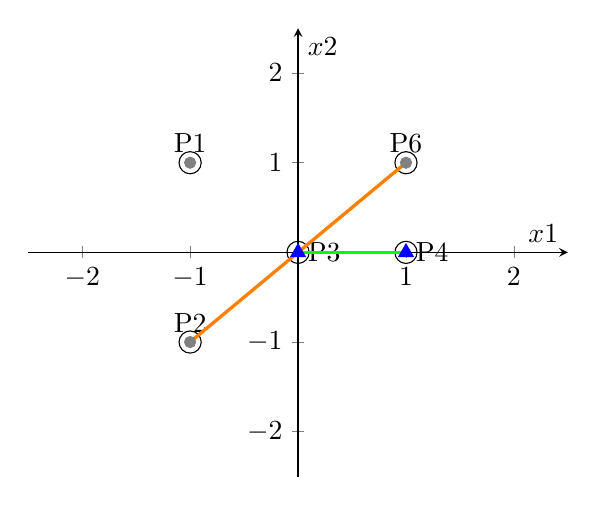
\begin{tikzpicture}
\begin{axis}[
    axis lines=middle,
    xmin=-2.5, xmax=2.5,
    ymin=-2.5, ymax=2.5,
    xlabel={$x1$},
    ylabel={$x2$}],
    
    ]


% \addplot[black](0.3,1.8) circle (0pt) node[anchor=west] {\large y=0 region};

\addplot[black](1,1) circle (4pt) node[anchor=south] {P6};


% #p1, p2,p6
\addplot[color=gray,only marks,] coordinates {(-1,1)(-1,-1)(1,1)};
% p3, p4
\addplot[color=blue, only marks, mark=triangle*,mark size = 3pt]coordinates{(0,0)};
\addplot[color=blue, only marks, mark=triangle*,mark size=3pt]coordinates{(1,0)};

\addplot[black](-1,1) circle (4pt) node[anchor=south] {P1};
\addplot[black](-1,-1) circle (4pt) node[anchor=south] {P2};
\addplot[black](0,0) circle (4pt) node[anchor=west] {P3};
\addplot[black](1,0) circle (4pt) node[anchor=west] {P4};

% The lines
\addplot [smooth,orange,name path=X,no marks,style=very thick]coordinates{(-1,-1)(0,0)(1,1)}; % actual curve
\addplot [smooth,green,name path=X,no marks,style=very thick]coordinates{(0,0)(0.5,0)(1,0)}; % actual curve
% \addplot [smooth,blue,name path=AA,no marks,style= dashed]coordinates{(-2.5,2.5)(-1,1)(0,0)(2.5,-2.5)}; % actual curve
% \addplot [smooth,blue,name path=AB,no marks,style= dashed]coordinates{(-2.5,-2.5)(0,0)(2.5,2.5)}; % actual curve
\end{axis}
\end{tikzpicture}
\end{center}
\end{minipage}


\end{document}